\title{Quadrupole Information for the M\o ller Polarimeter in Hall A}
\author{
        Donald Jones \\
        Temple University\\
 }
\date{\today}

\documentclass[12pt]{article}
\usepackage{hyperref}
\usepackage[english]{babel}
\usepackage{geometry} 
\geometry{letterpaper}
\usepackage[font=footnotesize]{caption}
\usepackage{fullpage}
\usepackage{placeins}
\usepackage{rotating}
\usepackage{graphicx}
\graphicspath{{figures/}}
\usepackage{amssymb}
\usepackage{amsmath}
\usepackage{color}
\usepackage{wrapfig}
\pagecolor{white}
\begin{document}
\maketitle

\begin{abstract}
This is intended to be a summary of the existing information for the Hall A M\o ller quadrupole magnets.
\end{abstract}

\section{Introduction}
The Hall A M\o ller polarimeter was originally designed with a magnetized Fe-foil target followed by a 3-quadrupole + dipole spectrometer focusing events onto a detector. Over the years modifications have been made to the target, the spectrometer and the detector package. The focus of this note is a summary of the quadrupoles. The information for this summary comes largely from \href{https://hallaweb.jlab.org/equipment/moller/spectrometer.html}{https://hallaweb.jlab.org/equipment/moller/spectrometer.html} and is meant to clarify what can be confusing and sometimes apparently conflicting information. 
\section{History}
The original quadrupole magnets used in the M\o ller polarimeter for Hall A came from LANL. Photocopies of documentation found at \\ \href{https://hallaweb.jlab.org/equipment/moller/magnets/Moller_quads2.pdf}{https://hallaweb.jlab.org/equipment/moller/magnets/Moller\_quads2.pdf} state that at least two of the quadrupoles were mapped originally in 1972, so we aren't dealing with new magnets. Four quadrupoles given the names Patsy, Jackie, Tessa and Felicia, were provided to Jefferson Lab by LANL for the Hall A M\o ller polarimeter. Only 3 were used in the original design since that was sufficient for the 6~GeV program. Jackie was in the worst shape and was put in storage. In 2012 a new fourth quadrupole magnet was designed to allow for the beam energies of the 12~GeV upgrade. Looking through the documentation can be confusing since these magnets were referred to differently depending on when the document was written and where they were placed on the beamline at the time. For example quadrupole 1 refers to Patsy in the 6~GeV era but generally is used to mean the new quadrupole after 2015. Some documents refer to a quadrupole 0. Table \ref{tab:nomen} is included to provide nomenclature reference.
\begin{table}[ht]
\begin{center}
\caption{\label{tab:nomen}Reference table providing changing nomenclature for the spectrometer quadrupoles. ``Eugene's Ref.'' refers to Eugene Chudakov's summary on the following webpage \href{https://hallaweb.jlab.org/equipment/moller/magnets/quad_summary_simul.html}{https://hallaweb.jlab.org/equipment/moller/magnets/quad\_summary\_simul.html}.}
\begin{tabular}{|c|c|c|c|}
\hline
12 GeV position&ID             &Name &Eugene's Ref.\\ \hline
Q1                     &QO1H01  &New    &Q4                  \\ \hline
Q2                     &QM1H02  &Patsy  &Q1                  \\ \hline
Q3                     &QO1H03  &Tessa  &Q2                  \\ \hline
Q4                     &QO1H03a&Felicia &Q3                  \\ \hline
\end{tabular}
\end{center}
\end{table}

Patsy and Jackie were identical magnets as were Tessa and Felicia. The new fourth quadrupole was designed to be similar to Tessa and Felicia, although it turned out to have larger contributions from higher multipole moments and. The physical information for the 4 quadrupoles (excluding Jackie) is provided in Table \ref{tab:quad_info}.

\begin{sidewaystable}[ht]
\begin{center}
\caption{\label{tab:quad_info}Physical parameters of the four quadrupole magnets.}
\begin{tabular}{|c|c|c|c|c|}
\hline
~                                &New             &Patsy                              &Tessa                            &Felicia\\ \hline
Manufacturer             &?                  &MagnaTek                       &Indust. Coil                   &Indust. Coil\\ \hline
Height (in)                  & ?                 &14 1/8                             &22 1/8                           &22 1/8\\ \hline
Width (in)                   &?                  &14 1/8                             &22 1/8                           &22 1/8\\ \hline
Length (in)                 &?                   &16                                  &12                                 &12\\ \hline
Effective Length (cm)&~                   &44.77 (1996)                  &36.74(1996)                  &36.6(1996)\\ 
~                                & 36.58(2015)&44.73 (2012)                   &~                                   &~\\ \hline
Bore/Aperture (in)      & 4.0              & 4.0                                 &4.0                                 &4.0\\ \hline
Max Current (A)         &280              &300                                 &280                                &280\\ \hline
Pole tip field               &--                 &0.5801(R=4.96 cm 1996)&0.6029(R=5.00 cm1996)&0.6135(R=5.00 cm1996)\\ 
@ 300 A (T)               &(2015)         &0.5604 (R=4.6 cm 2012)&~                                    &~\\ \hline
\end{tabular}
\end{center}
\end{sidewaystable}
\FloatBarrier
 Here are key points in the history I was able to piece together.
\begin{itemize}
\item{1972: Tessa and Felicia are mapped at LANL.}
\item{1996: Patsy, Jackie, Tessa and Felicia are all mapped at LANL before being given to JLab. Quadrupole and higher order multipoles are measured. The multipole measurements are recorded in an LANL document apparently first copied into a document at UK which was then poorly photocopied into the first 6 pages of document MiscQuadInfo.pdf. It appears pg.1 was written by someone at UK. Pages 2-6 contain photocopies of a LANL document with measurements recorded from 1996 and including some information on the plots on page 6 from 1972. Page 14 (labeled pg 1 of a document by Sirish Nanda made in 2000) appears to simply replicate the information in the tables of the LANL data in pages 2-3. It is not clear where the effective length values come from.}
\item{1997: Magnetic fields of Patsy, Tessa and Felicia remeasured by the University of Kentucky. Multipole components do not appear to be remeasured. The measurements at UK are not clearly labeled so it is difficult to know which ones they are. Perhaps the hysteresis curves shown on pages 15-19 of MiscQuadInfo.pdf. It is not clear what the information is on pages 7-12 of this document. Is it a UK measurement? There is a hand-written note saying these are from EPICS field maps. Not sure what to make of this. Regardless, pages 7-12 don't provide much additional information except to say the quads are essentially linear at the parts per thousand level up to 150 A or about half max.}
\item{1998: M\o ller polarimeter commissioned.}
\item{2012: Patsy removed from beam line and mapping performed by magnet group at Jefferson Lab. Multipoles and gradient measured.}
\item{2012: New 4th magnet (now Q1) manufactured similar in design to Tessa and Felicia.}
\item{2013: Four quadrupole configuration installed.}
\item{2015: 11~GeV beam tested in Hall A M\o ller}
\end{itemize}

Insights and questions from this history:
\begin{enumerate}
\item{All our information for the two most downstream quadrupoles are from decades ago. To what accuracy were they mapped and can we still trust the decades old information?}
\item{Patsy was remeasured in 2012. How consistent were those results with the 1996 and 2000 maps?}
\item{The new quadrupole was mapped most recently. How well do we know that mapping?}
\end{enumerate}
We will address these questions individually in the sections ahead.


\section{New quadrupole (Q1 or QO1H01)}
The new quadrupole was mapped in 2012. The raw data is found in the spreadsheet QO1H01\_Summary1.xlsx. Four (at least) different data sets were taken.

\subsection{Effective length}
Effective length was measured moving a Hall probe along Z at R=4.035~cm. The effective length was found to be 36.58~cm and the value at the center (Z=0) was 0.51404 T. The data are shown in Fig. \ref{fig:Q1_eff_len}.
\begin{figure}[!h]
\centering
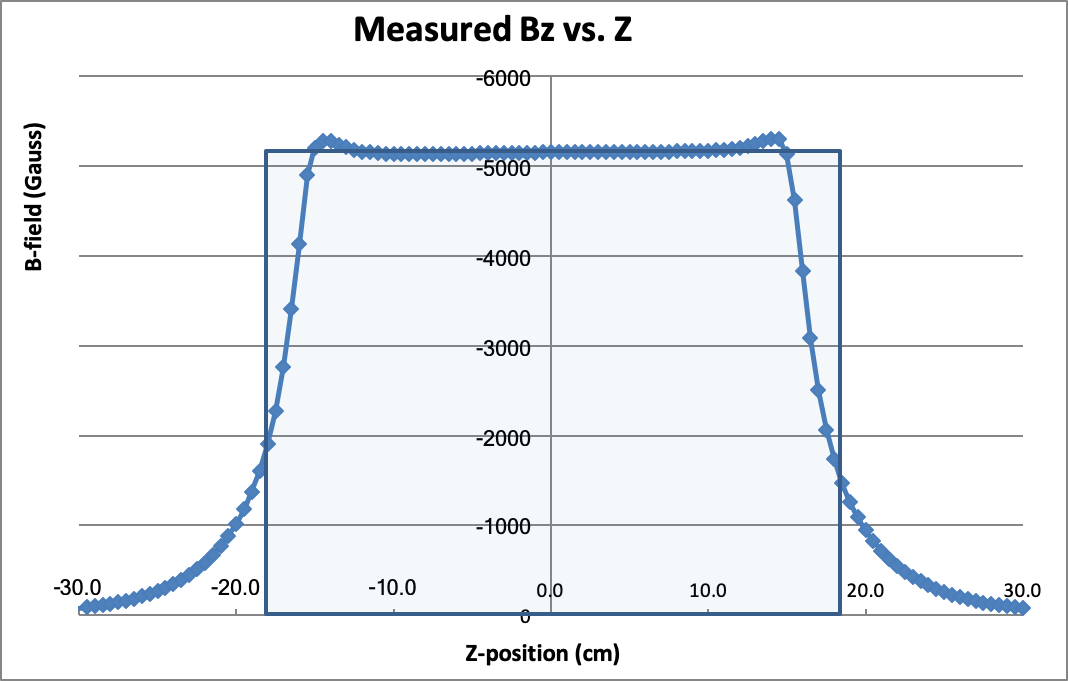
\includegraphics[width=0.6\textwidth]{QO1H01_Eff_Len.png}
\caption{\label{fig:Q1_eff_len}Hall probe measurements taken along Z for QO1H01 at r=4.035~cm. The effective length, 36.58~cm, is shown as the shaded region.}
\end{figure}

\subsection{Harmonics: multipole expansion}
The magnetic field in a region free of current can be approximated in a truncated multipole expansion. For cylindrical coordinates the radial,$B_r$and azimuthal, $B_{\phi}$ components of the field can be expressed in terms of sines and cosines as
\begin{align*}
B_r&=\sum_nA_n\left(\frac{r}{r_0}\right)^{n-1}\sin\left(n\phi-\alpha_n\right), ~~~~n=1,2... \\
B_{\phi}&=\sum_nA_n\left(\frac{r}{r_0}\right)^{n-1}\cos\left(n\phi-\alpha_n\right),
%\label{eq:harmonics}
\end{align*}
where $A_n$ are constant coefficients dictating the relative strength of the contributions. $\alpha_n$ is an offset term in case the coordinate system has an offset azimuthal angle relative to the field axes. The index $n$ gives the multipole order. $n=2$ gives the quadrupole term with 2 negative and 2 positive poles in the azimuth and is proportional to $r$. To determine the harmonics of the magnetic field a wire coil of radius 3.699~cm rotating at a fixed frequency was used. The signal from the coil was analyzed using a lock-in amplifier to pick out the harmonics. The coil had a radius of 3.699~cm whereas the pole tip is at 5.08~cm. 
Only the n=2 (quadrupole) and n=6 (dodecapole) contributions were measured to be significant as can be seen in Table \ref{tab:q1_harmonics}. The n=6 contribution was found to be 1.44\% of the quadrupole at R=3.699~cm. Since the dodecapole depends on the $r^5$ whereas the quadrupole on $r$ this translates into a n=6 contribution of 5.12\% at the pole tip. 

\begin{table}[!h]
\begin{center}
\caption{\label{tab:q1_harmonics}Newest quadrupole (QOH01) showing the harmonic multipole contributions relative to the quadrupole contribution measured at $r=3.699$~cm. Multipoles up to n=20 were measured. Shown here are all harmonic contributions above 0.01\% of the quadrupole.}
\begin{tabular}{|c|c|c|c|c|c|c|c|}\hline
Current & n=2           &n=3 & n=4 & n=5 & n=6    & n=7  & n=10\\
(A)        & (arb)          &(\%) & (\%)& (\%) & (\%)   & (\%)  & (\%) \\\hline
100.0    &44217.253 &0.035&0.035&0.114&1.438&0.012&0.056\\\hline
200.0    &87505.650 &0.035&0.036&0.116&1.439&0.012&0.056\\\hline
300.0    &118079.471&0.035&0.036&0.116&1.441&0.012&0.056\\\hline
\end{tabular}
\end{center}
\end{table}
\subsection{Gradient-length (GL)}
GL measurement versus current from -300~A to 300~A using a stretched wire to determine the non-linearity of the quadrupole from saturation. 
\subsection{Map of Bdl}
A map of Bdl was made using a stretched wire at 5 different X-positions and at 22 different currents ranging from -300~A to 300~A. These data were also analyzed to assess the multipole components. The full map can be found in QO1H01\_Summary1.xlsx. 

In Eugene's quadrupole summary page an analysis of these data was performed. Using the rotating coil analysis, tthe contribution of n=6 was fixed at 4.8\% at r=5~cm and GL and an X-offset were allowed as fit parameters (see the following webpage: \href{https://hallaweb.jlab.org/equipment/moller/magnets/quad_summary_simul.html}{https://hallaweb.jlab.org/equipment/moller/magnets/quad\_summary\_simul.html}). The fits to the data have rather apparent large residuals although they are not tabulated and the X-offset was found to be 0.4~mm. GL was found to be 4.76~T at 300~A. I was not able to replicate these results using the same data. Figure \ref{fig:EugeneComp} shows the fits and residuals following the same procedure. I find much better agreement with data (small residuals), an X-offset of $7\pm27~\mu$m consistent with zero and a GL at 300~A of 4.72~T. The source of these discrepancies is not clear.
\begin{figure}[!h]
\centering
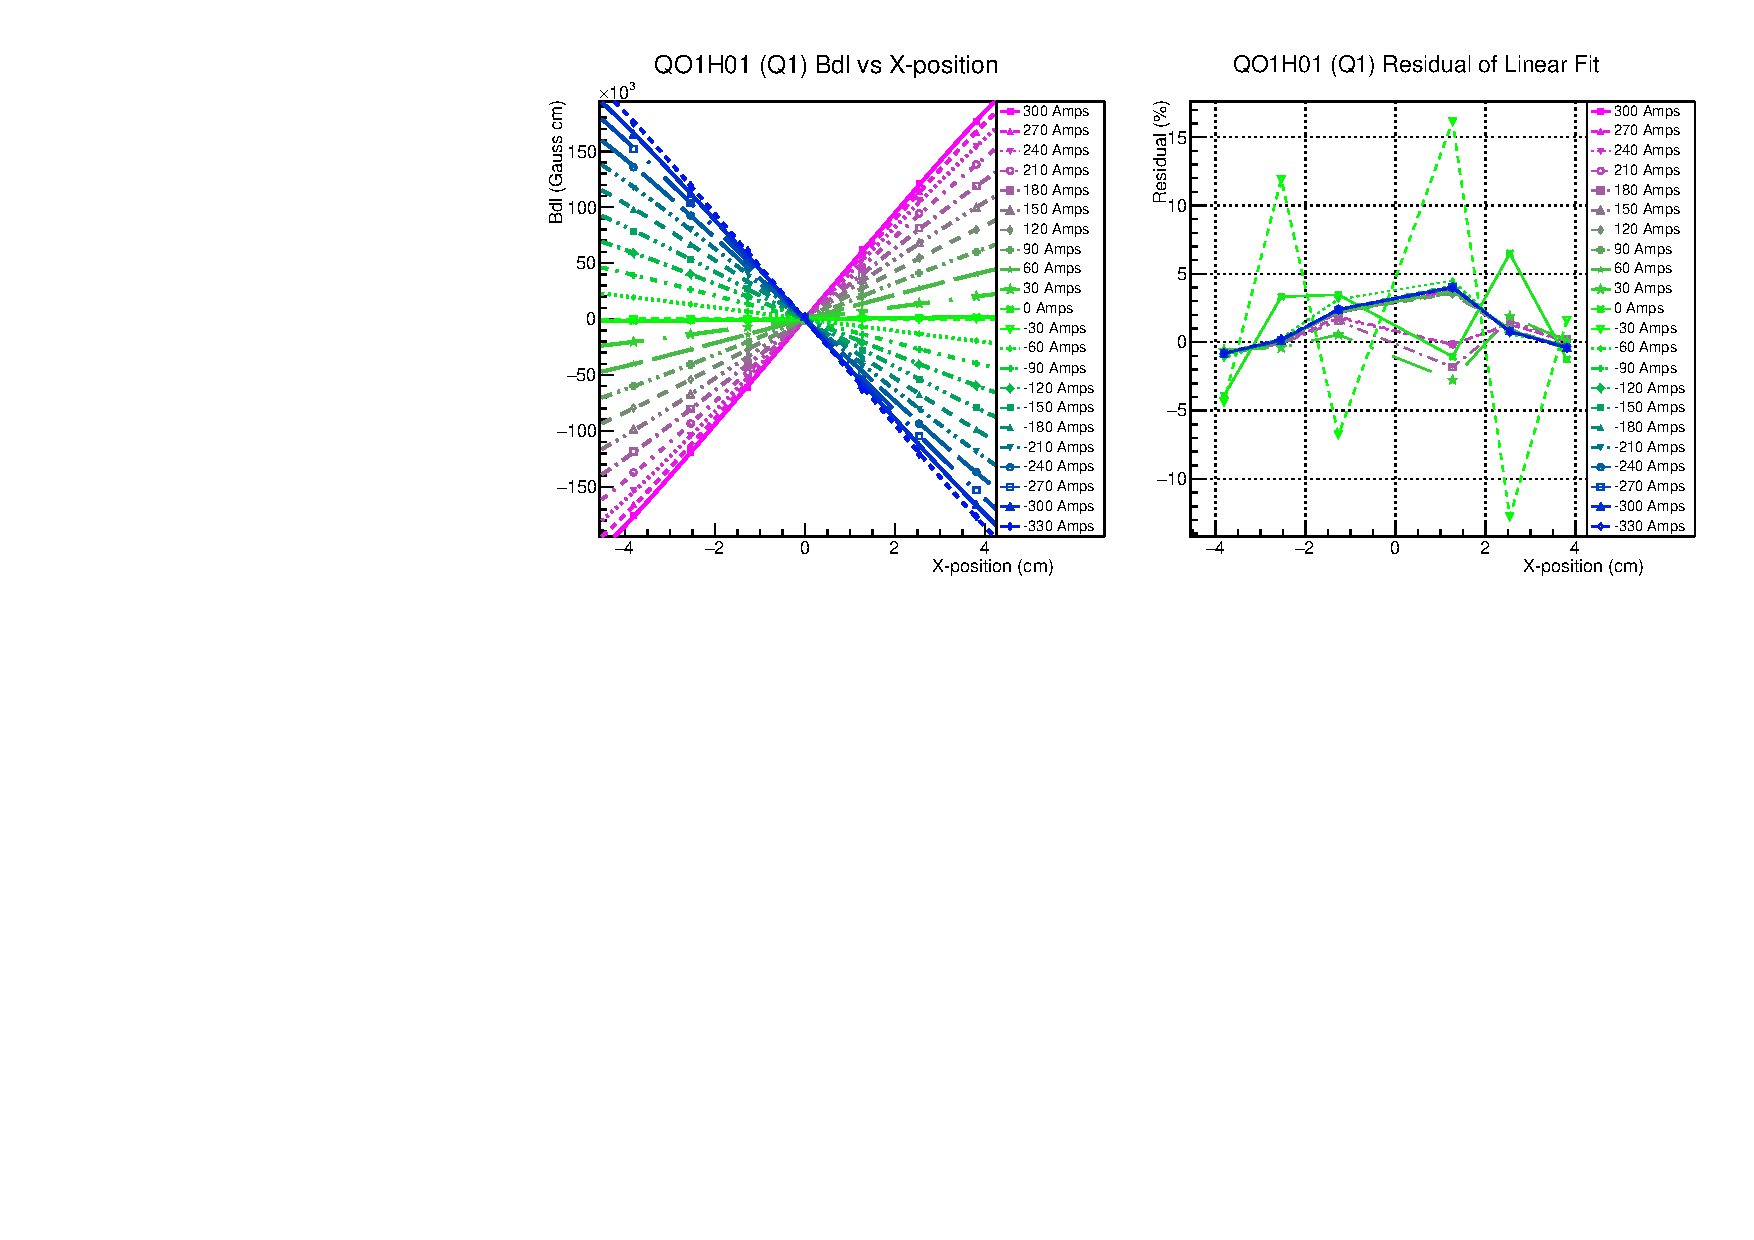
\includegraphics[width=1\textwidth]{EugeneCompNewQ1.pdf}
\caption{\label{fig:EugeneComp}Attempted replicated of Eugene's results fixing the contribution of n=6 to 4.8\% at r=5~cm. QO1H01 Bdl measurements for 5 different X-positions and 22 currents. The following fit equation is utilized where square brackets indicate fit parameters: $Bdl=[GL](x-[x_0])\left(1-0.048\left(\frac{x-[x_0]}{5.0}\right)^4\right)$.}
\end{figure}

Redoing the analysis, but allowing the n=6 contribution to be a fit parameter gives improved results. I did not find that allowing other multipole contributions than quadrupole and dodecapole improved the $\chi^2/NDF$ significantly, but rather made the fits unstable. The improved results are shown in Fig. \ref{fig:Q1_BdlvsX}. With the exception of low current data where the small denominator produces large fluctuations, residuals are less than $\pm$3\% and generally much less than this. 
\begin{figure}[!hb]
\centering
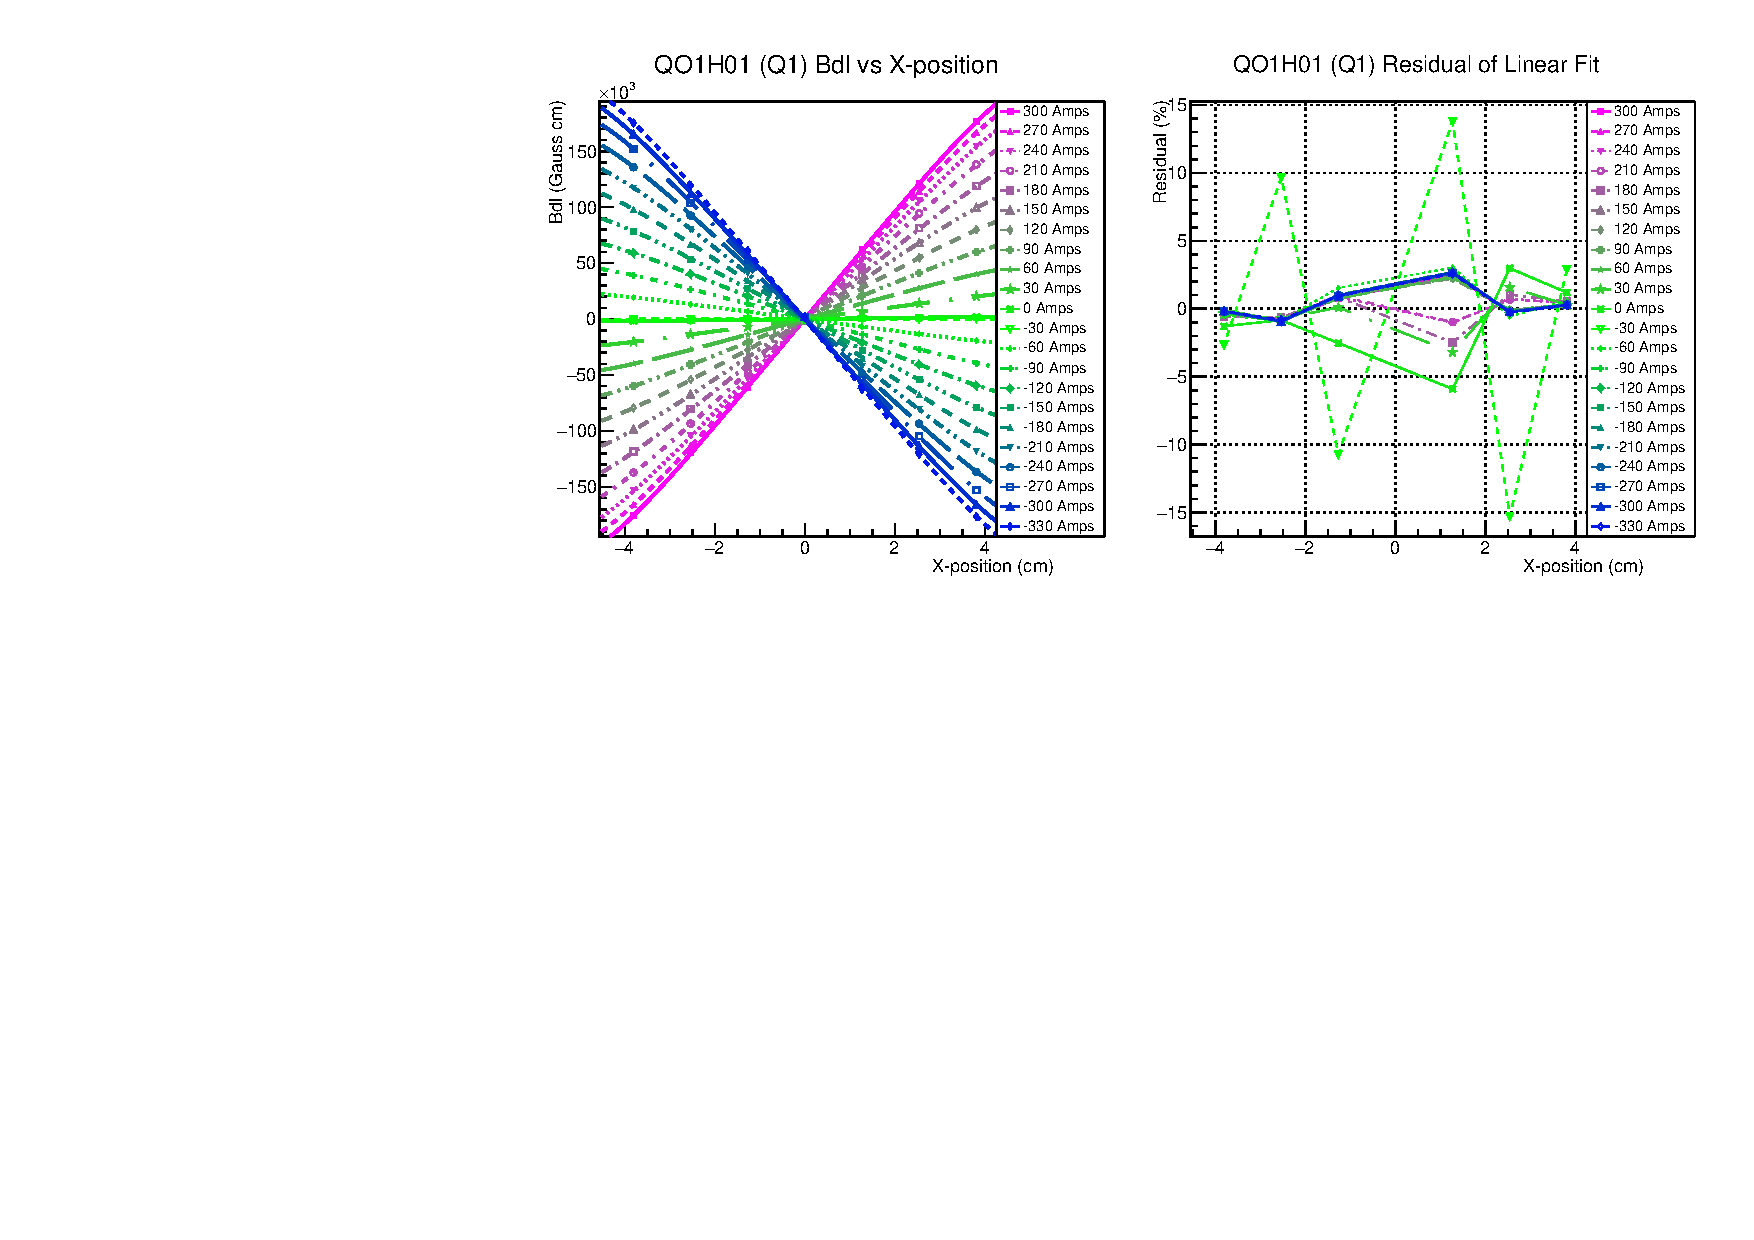
\includegraphics[width=1\textwidth]{QO1H01_BdlvsX.pdf}
\caption{\label{fig:Q1_BdlvsX}QO1H01 Bdl measurements for 5 different X-positions and 22 currents allowing the n=6 contribution to come from the fit. The following fit equation is utilized where square brackets indicate fit parameters: $Bdl=[GL](x-[x_0])\left(1-[A_6]\left(\frac{x-[x_0]}{5.08}\right)^4\right)$.}
\end{figure}
Table \ref{tab:q1_multipole} gives the fit results for the X-offset and n=6 relative contribution. Once again a negligible offset is assessed at $20\pm30~\mu$m. The dodecapole contribution is favored to be much larger (around 12\%) than that found by the rotating coil. \textbf{This suggests that we need to include the dodecapole in the simulation and that there may be some flexibility in adjusting its relative contribution.}

\begin{table}[ht]
\begin{center}
\caption{\label{tab:q1_multipole}Newest quadrupole (QOH01) offset and n=6 multipole fractional component as determined from fitting the gradient-length versus X-position data at 22 different currents. These are the fit results shown in Fig \ref{fig:Q1_BdlvsX}. These are extrapolated to the pole tip at R=5.08~cm. The average dodecapole contribution is about 12\%, more than double that assessed by the rotating coil analysis.} 
\begin{tabular}{|c|c|c|}\hline
Current &Offset & Dodecapole \\ 
(A)     &(mm)   &Coeff (frac)\\ \hline 
  300.0 & -0.06 &     -0.114 \\ \hline
  270.0 & -0.04 &     -0.114 \\ \hline
  240.0 &  0.04 &     -0.091 \\ \hline
  210.0 &  0.05 &     -0.091 \\ \hline
  180.0 &  0.08 &     -0.082 \\ \hline
  150.0 & -0.04 &     -0.111 \\ \hline
  120.0 & -0.05 &     -0.114 \\ \hline
   90.0 & -0.03 &     -0.114 \\ \hline
   60.0 & -0.04 &     -0.117 \\ \hline
   30.0 &  0.12 &     -0.071 \\ \hline
    0.0 &  0.31 &     -0.289 \\ \hline
  -30.0 &  0.57 &     -0.196 \\ \hline
  -60.0 & -0.02 &     -0.123 \\ \hline
  -90.0 & -0.06 &     -0.118 \\ \hline
 -120.0 & -0.06 &     -0.112 \\ \hline
 -150.0 & -0.05 &     -0.115 \\ \hline
 -180.0 & -0.05 &     -0.115 \\ \hline
 -210.0 & -0.06 &     -0.115 \\ \hline
 -240.0 & -0.06 &     -0.115 \\ \hline
 -270.0 & -0.06 &     -0.117 \\ \hline
 -300.0 & -0.06 &     -0.116 \\ \hline
 -330.0 & -0.08 &     -0.117 \\ \hline
\hline
Average &  0.02 &     -0.121 \\ \hline 
\end{tabular}
\end{center}
\end{table}

\section{Patsy (Q2 or QM1H02)}
Patsy is the most linear quadrupole of the four w.r.t. current meaning it suffers least from saturation effects at higher currents. Patsy was measured in 1996 at LANL and its GL and pole tip field measured versus current and its multipoles contributions measured. In 1997, the hysteresis curves were measured at the University of Kentucky. The results can be found in MiscQuadInfo.pdf as well. These were also transcribed in 2020 into the spreadsheet quadrupole\_info.xlsx and can be found in Table \ref{}.


Figure \ref{fig:Patsy2012} shows the results of the most recent measurement as well as a 5-deg polynomial fit and the existing 5-deg polynomial parametrization used in the GEANT4 simulation. The new parametrization does a better job at low currents and the two are equivalent at currents above $\pm$150~A. This new parametrization is recommended.

Fig. \ref{fig:Pasty2012UKcomp} shows a comparison of the 2012 JLab and 1997 UK measurements of Q2 (Patsy) GL versus current along with 5 degree parametrizations for each data set. The absolute difference $\times100$ between the 2012 parametrization and the 1997 measurements shows differences ranging from -0.08~T to +0.05~T. The percent difference between the two parametrizations is also shown and varies from several percent at low current to about 1\% near the maximum. The reason for these differences is not clear. Are they real or the result of measurement error? No matter how they arise, they suggest that the uncertainty in the magnetic field of Q2 is at the level of a 1-2\% at high current and larger at lower current.
 \begin{figure}[!h]
\centering
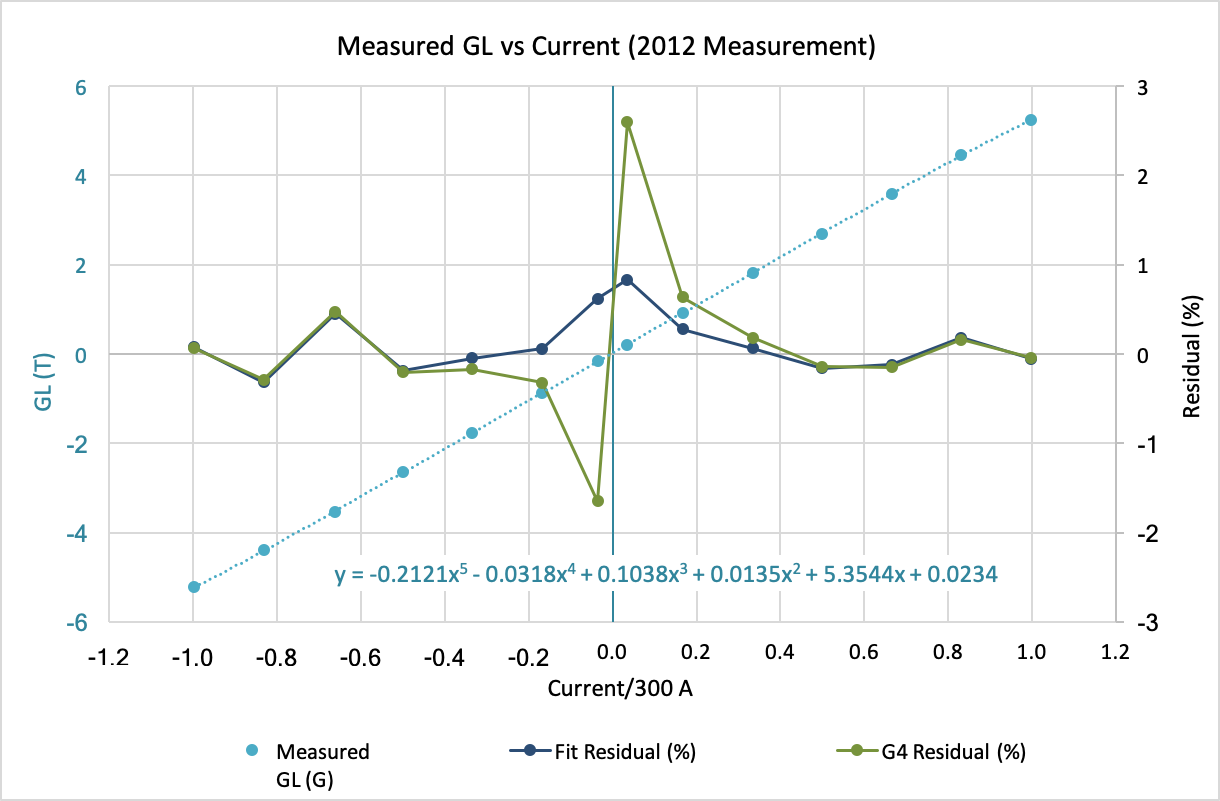
\includegraphics[width=0.8\textwidth]{Patsy2012.png}
\caption{\label{fig:Pasty2012} Results of the 2012 JLab measurement of Q2 (Patsy) GL versus current. A 5 degree polynomial parameterization is shown along with the existing parametrization in G4. The new parametrization is better at low currents less than 100 A but is essentially identical above this.}
\end{figure}
\begin{figure}[!h]
\centering
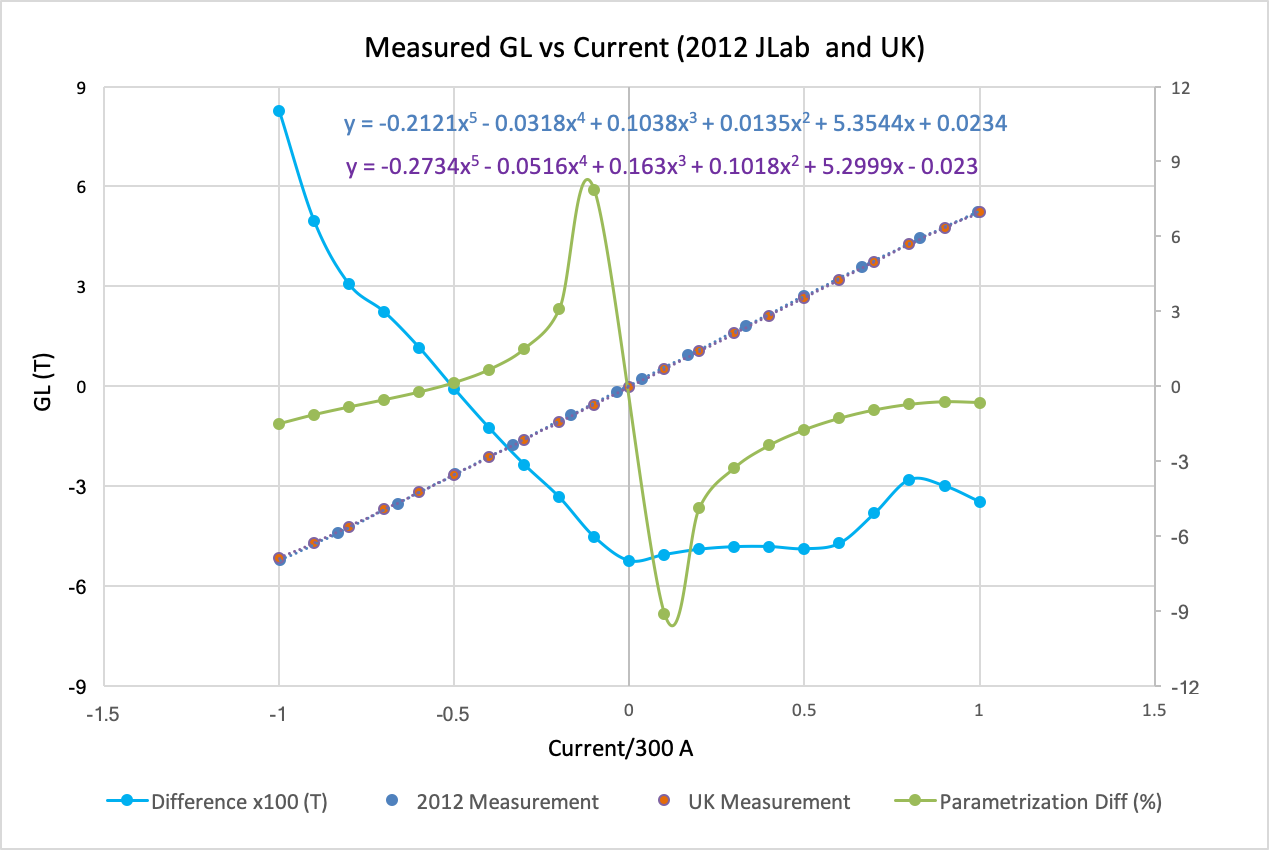
\includegraphics[width=0.8\textwidth]{Patsy2012UKcomp.png}
\caption{\label{fig:Pasty2012UKcomp} Comparison of the 2012 JLab and 1997 UK measurements of Q2 (Patsy) GL versus current. 5 degree parametrizations are also shown for each data set. Since the data sets are taken at different current comparisons were made using the parametrizations where required. The absolute difference $\times100$ between the 2012 parametrization and the 1997 measurements shows differences ranging from -0.05~T to +0.08~T. The percent difference between the two parametrizations is also shown.}
\end{figure}
%\bibliographystyle{abbrv}
\bibliographystyle{unsrt}
\bibliography{bibliography}

\end{document}
